\section{Result section title}
MSE, PCA, R2, compair.
Ordered by target:
 
\subsection{Random factors from database.}
\subsubsection{Average Voltage}
\subsubsection{Capacity}
\subsubsection{Energy Density}

\subsection{Volumetric number density}

\begin{figure}
\begin{tabular}{|c|c|c|c|c|c|}
	\hline 
	 $\frac{Target:}{Accuracy:}$& Average Voltage & Gravimetric Capacity & Volumetric Capacity & Specific Energy & Energy Density $\si{Wh/kg}$ $\si{Wh/l}$ \\ 
	\hline
	$R^2$-score & -0.0461 & 0.3426 & 0.3784 & -0.0011 & 0.0838\\ 
	\hline 
	$R^2$-train & 0.8676 & 0.8799 & 0.9052 & 0.8764 & 0.8786 \\ 
	\hline 
	CV: & -0.7976(+/- 1.3547)& 0.1844 (+/- 0.2182) & 0.2983 (+/- 0.3636) & -0.3742 (+/- 0.9904) & -0.1623 (+/- 0.7009) \\ 
	\hline
	MSE: & 1.1457 & 4521.6902 & 62785.2 & 92593.3 & 1613762.6538 \\ 
	\hline
	CV-mean: &-0.5899 & 0.1660 & 0.3166  &-0.2962 &-0.0398 \\
	\hline
\end{tabular}
\caption{Wall of numbers.}
\end{figure}


\subsubsection{Average Voltage}
Charged:

Discharged:

\subsubsection{Capacity}

\subsubsection{Energy Density}


\subsection{Void fraction}
%\subsubsection{Average Voltage}
%\subsubsection{Capacity}
%\subsubsection{Energy Density}







\subsection{AP-RDF}
PCA, R2, MSE.

\subsection{Stability}







%Preliminary Results: 
This is a novel work, the aim is therefor to explore different predictors, by figuring out the different weights of the predictors on different targets, and which predictors that does not favorable for our predictions. 

The model is decent at predicting; Gravimetric and Volumetric Capacity($87\%$), Specific Energy($70\%$), and Energy density($68\%$), but has no capability of predicting stability as of now. There is a need for \textit{ab initio} calculations for several of our predictors, they calculate something that we know most definitely is correlated to the target without any premature calculations. This is something we are trying to move away from. As of now, only using the density fraction, we can get somewhere between $40 \%$ to $60 \%$ accuracy with our model. 

This did not improve when including the void fraction, our predicitons actually got worse.   

AP-RDF - Still no good results! \myworries{This is a struggle.}


\subsection{Geometrical descriptors}
These grafs all represent the accuracy of the predictions on the training data and on new data given to the machine, with only the number density as a predictor, and the Average voltage, Gravimetric capacity, Volumetric capacity, energy density, and physical stability for the discharged material, as targets (a-f)\ref{fig:numberdensity_a-f}. Most notably the predictions on the Average voltage, Gravimetric capacity, Volumetric capacity, energy density, and specific energy are all showing a decent amount of correlation, with around $60\%$ accuracy. 
The physical stability for the discharged-,and the physical stability of the charged-materials show that there is no correlation between the number density and the physical stability. 
It is also shown that there is no correlation between the number density and the void fraction. Or any of the other properties for that matter. 


\begin{comment}
\begin{figure}[H]
    \centering
    \begin{subfigure}{0.3\textwidth}
        \centering
        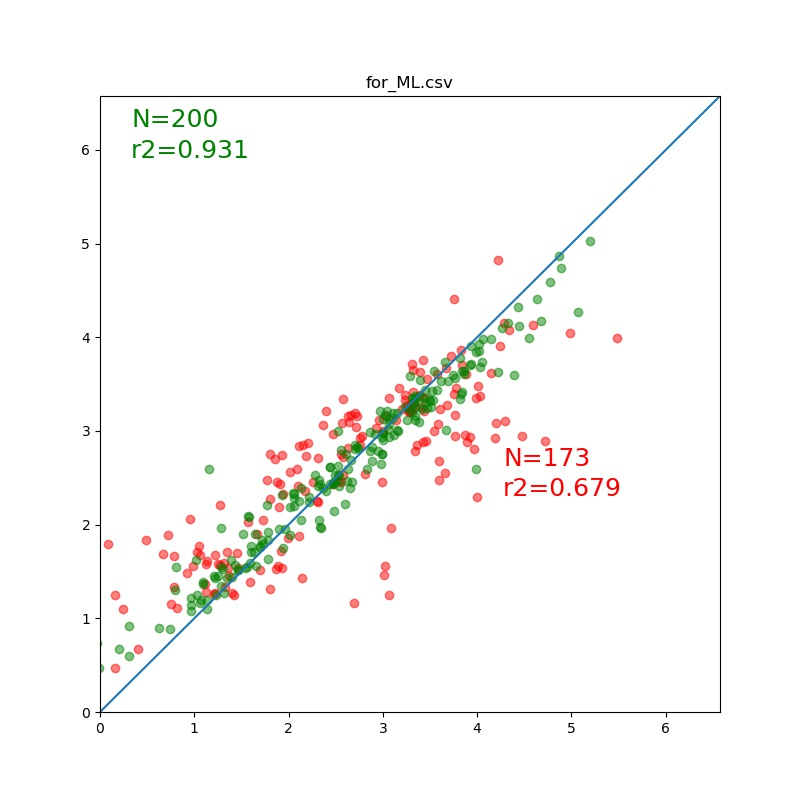
\includegraphics[width=\linewidth]{Results/2019-04-11/target=Average_Voltage.jpg}
        \caption{}
    \end{subfigure}
   % ~ 
    \begin{subfigure}{0.3\textwidth}
        \centering
        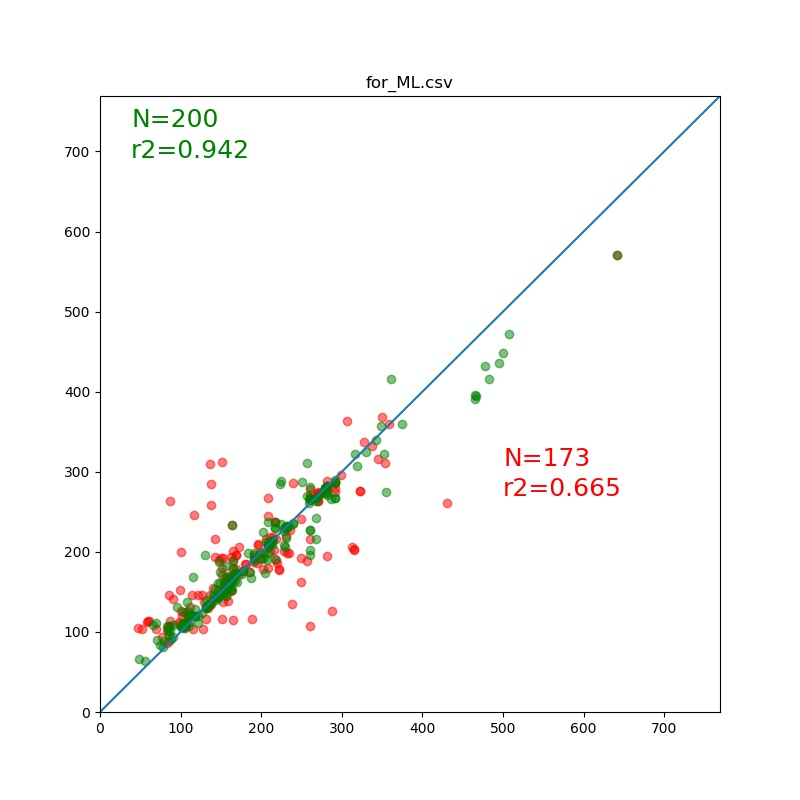
\includegraphics[width=\linewidth]{Results/2019-04-11/target=Capacity_Grav.jpg}
        \caption{}
    \end{subfigure}
       % ~ 
    \begin{subfigure}{0.3\textwidth}
        \centering
        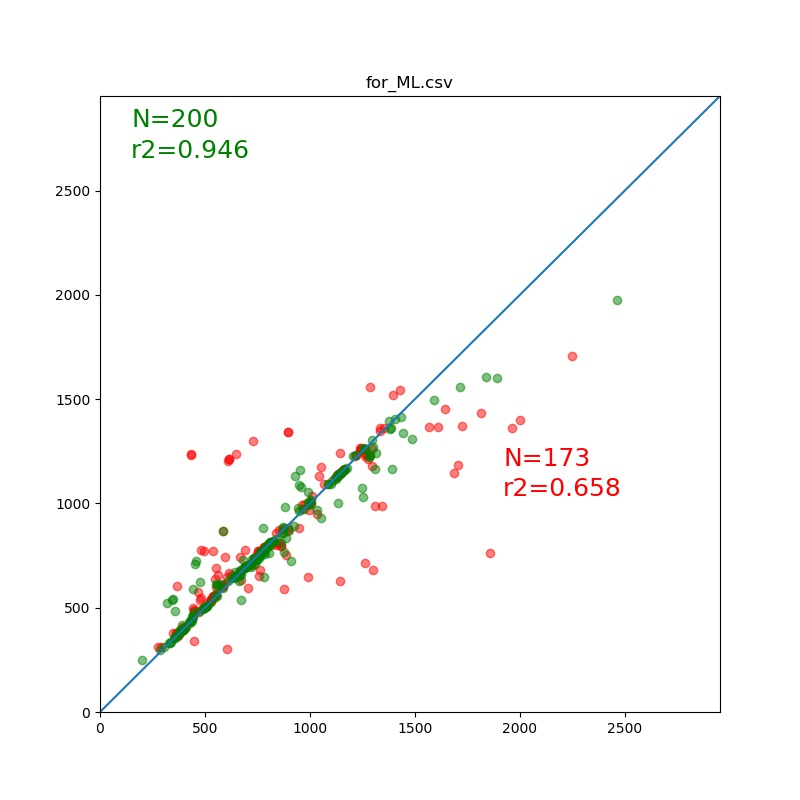
\includegraphics[width=\linewidth]{Results/2019-04-11/target=Capacity_Vol.jpg}
        \caption{}
    \end{subfigure}
       % ~ 
    \begin{subfigure}{0.3\textwidth}
        \centering
        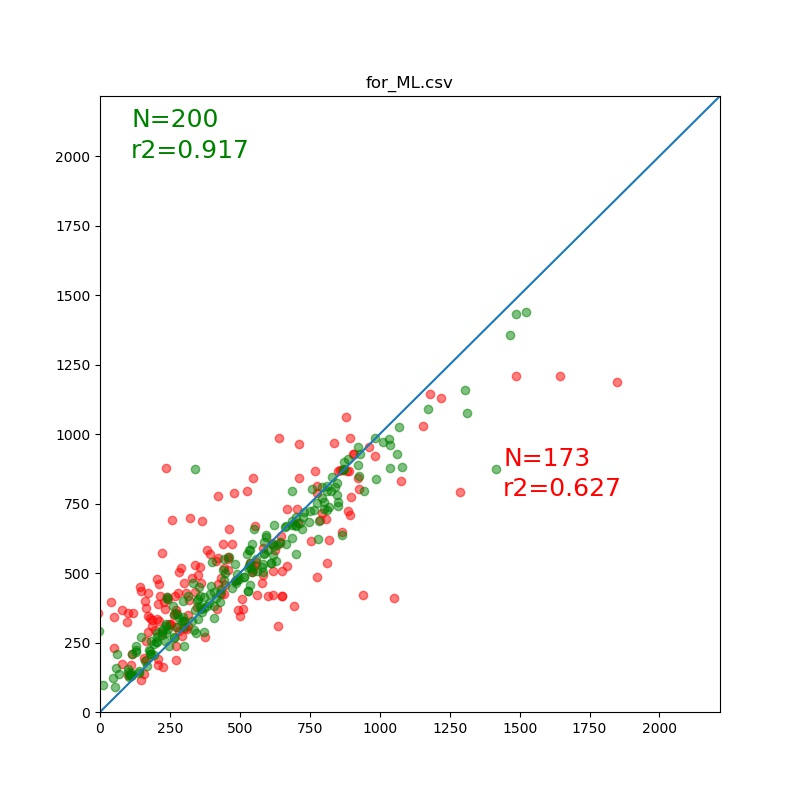
\includegraphics[width=\linewidth]{Results/2019-04-11/target=Specific_E_Wh_kg.jpg}
        \caption{}
    \end{subfigure}
       % ~ 
    \begin{subfigure}{0.3\textwidth}
        \centering
        \includegraphics[width=\linewidth]{Results/2019-04-11/target=E_Density_Wh_l.jpg}
            \caption{}
    \end{subfigure}
       % ~ 
    \begin{subfigure}{0.3\textwidth}
        \centering
        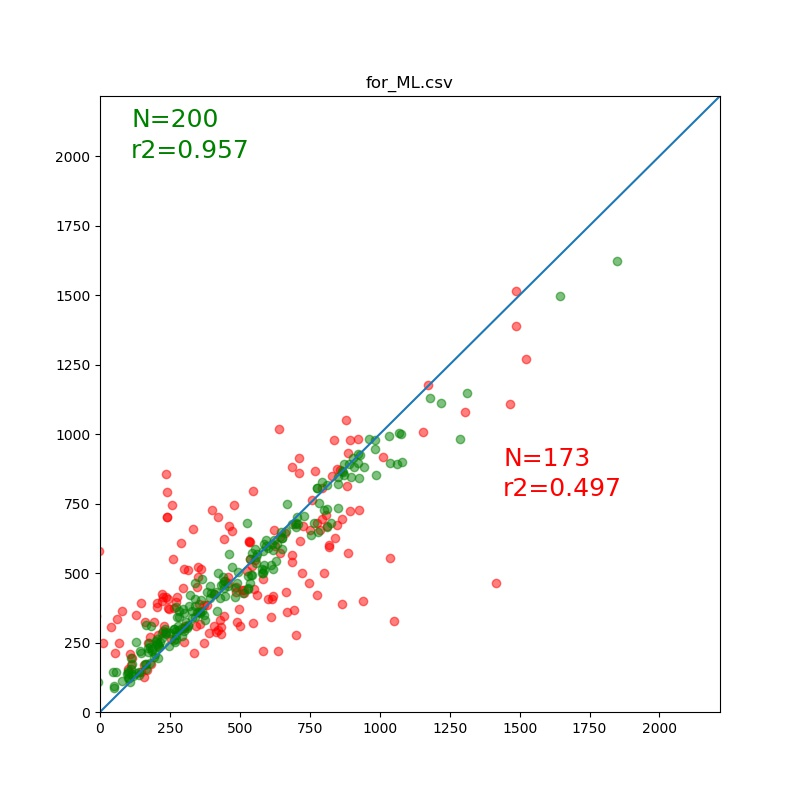
\includegraphics[width=\linewidth]{Results/2019-04-11/target=Stability_Discharge.jpg}
            \caption{}
    \end{subfigure}
\caption[R2 plot]{R2 plot for different runs}
    \label{fig:numberdensity_a-f}

\end{figure}

\subsection{Energy descriptions}

\begin{figure}
    \centering
    \includegraphics[width=\linewidth]{Results/plots/mean_crossvalidation_plot.png}
\caption[Cross validation and prediction uncertainty plot]{The Cross validation and the predictions uncertainty plottet for different runs with different predictors and the specific energy as the target for all runs. No removal of outliers have been implemented. l = number density, hgv = helvol, geomvol of void fraction, AV = average voltage, CGV = gravimetric and volumetric capacity, ED = energy density}
\label{fig:mean_cv}
\end{figure}
\myworries{}
\end{comment}


%Parameters.
%Volume number density
%Try to tell a STORY.


%Presentation between 30-45 minuttes. 

%Problem?
%method
%solution? 

% Test with density fraction:


% Test; weight of different parameters.















